\section{Architettura}

Per l'architettura dell'applicativo da sviluppare si è deciso di utilizzare
\textit{Model-View-ViewModel}, derivato da \textit{Model-View-Controller}.

\subsection{Viste}
% TODO: Viste non nel senso del pattern
Per garantire l'uniformità e la riusabilità di tutti i componenti delle varie
viste si è deciso di utilizzare per tutti la stessa struttura.

\subsubsection{Caratterizzazione di una vista}
Una vista è caratterizzata da:
\begin{itemize}
  \item Tipo di grafico (scatterplot, parallel coordinates, ecc...).
  \item Impostazioni di rendering.
  \item Associazione degli assi alle dimensioni del grafico.
\end{itemize}

\subsubsection{Logica di Rendering}
\begin{itemize}
  \item Renderer: componente che si occupa di adattare (Adapter pattern) il
    meccanismo di rendering delle varie librerie alla nostra architettura
    specifica, in particolare esso opera sui nostri oggetti di dominio come il
    dataset$^{G}$ già preparato per il render$^{G}$ (ad esempio mappati come punti 2
    dimensionali nello scatterplot$^{G}$) e le sue impostazioni specifiche di
    rendering$^{G}$ (ad esempio lunghezza degli assi x ed y nello scatterplot$^{G}$)
    traducendoli in un formato comprensibile dalla libreria di supporto.
  \item Mapper: componente che si occupa di trasformare il dataset$^{G}$ generale nel
    dataset$^{G}$ preparato per il render$^{G}$.
\end{itemize}

\begin{figure}[h!]
  \centering
  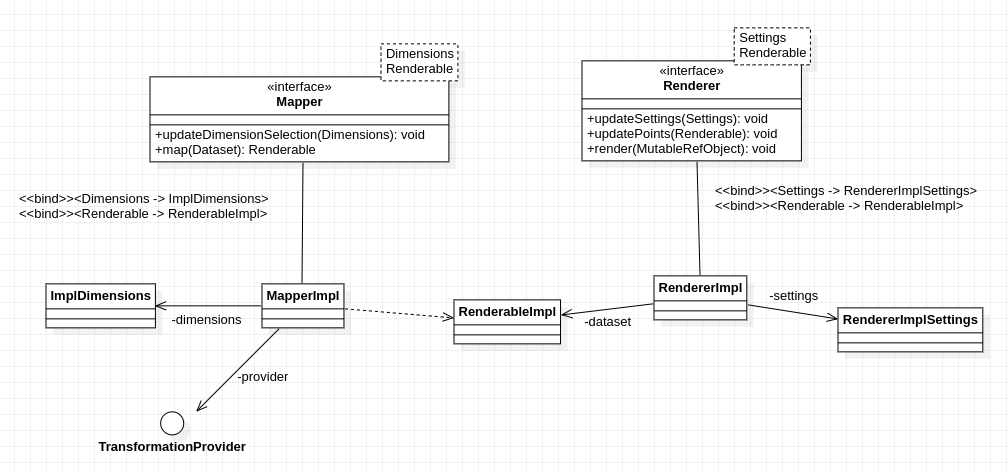
\includegraphics[scale=0.60]{../../assets/classi_uml/modelvista.png}
  \caption{Esempio di implementazione di una vista di tipo \texttt{Impl}.}
\end{figure}
\newpage
\subsubsection{Interazione con l'utente}
L'utente deve poter interagire con l'applicazione per poter modificare
preferenze del grafico specifico, quindi si utilizza mvvm per modellare questa
interazione. Il componente verrà generato utilizzando la libreria \texttt{MobX}.

\begin{figure}[h!]
  \centering
  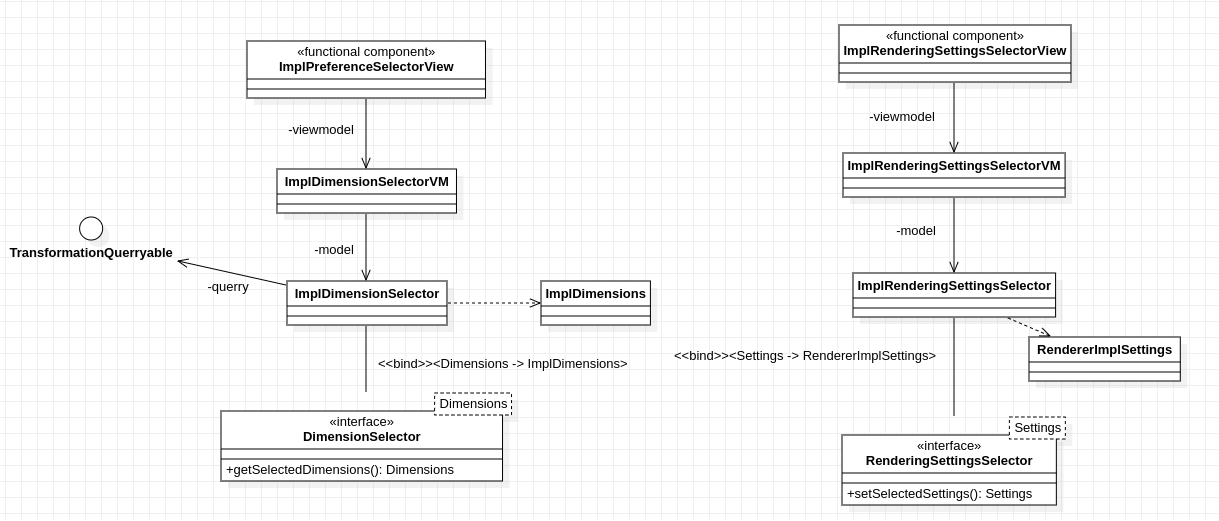
\includegraphics[scale=0.55]{../../assets/classi_uml/modelinterazione.png}
  \caption{Esempio di implementazione dell'interazione di tipo \texttt{Impl}.}
\end{figure}

\subsubsection{Composizione}
Per creare una vista completa sì utilizzerà un componente generico in modo da
favorire la composizione e creazione di nuove tipologie di vista, senza dover
interagire con il codice che si occupa di manipolare il flusso dei dati che vista
la nostra architettura risulta essere standard, senza perdere di flessibilità.

\begin{figure}[h!]
  \centering
  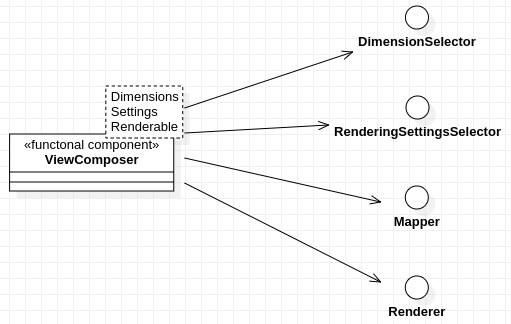
\includegraphics[scale=0.55]{../../assets/classi_uml/comdelcomposer.png}
  \caption{Dimostrazione di composizione generica}
\end{figure}

Il view composer date delle higher-order functions in grado di costruire i vari
componenti necessari, le preferenze, le dimensioni, un riferimento al dataset e
un riferimento al transformer sarà in grado di posizionare tutti i componenti
necessari per l'intreazione con l'utente ed effettuare il rendering della vista
e di orchestrarli quando avviene un cambiamento.

\begin{figure}[h!]
  \centering
  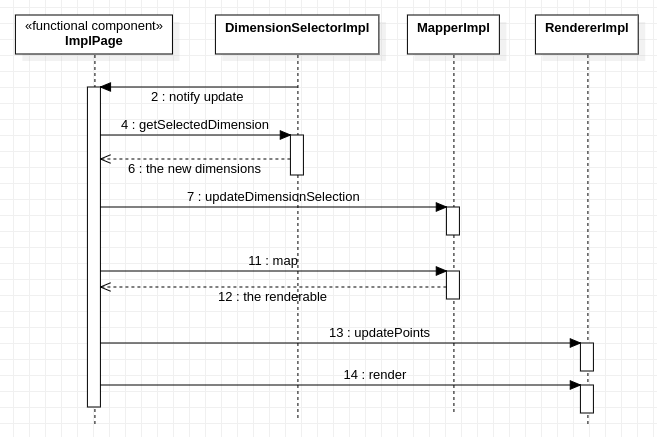
\includegraphics[scale=0.55]{../../assets/classi_uml/interazione_gw.png}
  \caption{Dimostrazione dell'orchestrazione dell' aggiornamento delle
    dimensioni da parte di generic view, ovviamente per semplcità è stato
    trattato dimension selector come un unico componente}
\end{figure}

\subsection{Stato dell' applicazione}
L'applicazione ha uno stato con cui tutte le viste interagiscono.
\begin{itemize}
  \item Viste create dall'utente in precedenza.
  \item Trasformazioni sui dati disponibili.
  \item Dataset$^{G}$.
\end{itemize}

\subsubsection{Trasformazioni}
Il transformer è la classe che mantiene traccia di tutte le trasformazioni (cioè
funzioni che trasformano un campo di una entry del dataset in qualcosa che il
renderer è in grado di disegnare). \\
Esso espone 2 interfacce così da segregarne l'uso, una è destinata alla ricerca di
trasformazioni (TransformationQuerryable) e l'altra al riferimento delle stesse tramite
signature (TransformationProvider).
\begin{figure}[h!]
  \centering
  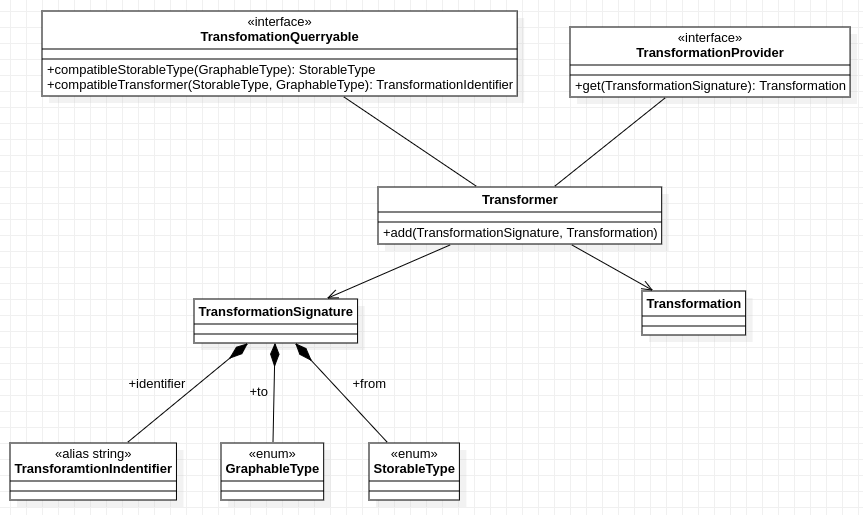
\includegraphics[scale=0.65]{../../assets/classi_uml/modeltransfomer.png}
\end{figure}

\subsubsection{Dataset}
Il dataset$^{G}$ raggruppa i dati caricati dall'utente in una collezione di
\texttt{DatasetEntry} che non sono altro che una collezione di coppie nome del
campo e valore (uno storable type). \\

\noindent
Il dataset non è altro che un insieme di \texttt{DatasetEntry} che rappresentano
una riga del dataset in un qualsiasi momento dell' elaborazione, una entry è un
insieme di field accompagnati dal loro tipo così da poter mostrare all'utente
solo opzioni sensate di rendering all'utente, il dataset espone la sua signature
cioè i suoi campi e loro tipo così da permettere introspezione su di esso.\\

\noindent
Per mettere l'estrazione di dati derivati il dataset espone un metodo di map,
simile a quello presente sulle varie collezioni standard inJavaScript/Typescript,
è possibile attivare o disattivare il check della signature del dataset.

\paragraph{Parsing del Dataset:}
Per rendere l'applicazione il più agnostica possibile al formato del dataset
(questo può tornare utile in caso si trovino altri dataset interessanti nella
fase esplorativa ed è praticamente gratis da implementare) si è deciso di
nascondere l'operazione dietro una interfaccia \texttt{DatasetParser}, questo
tipo di architettura risulterà anche molto flessibile in quanto potrà anche
essere parallelizzata facilmente in formati in cui il contesto è la singola
linea tipo \texttt{CSV} aggregandone più diversi.

\paragraph{Caricamento del Dataset:}
Sempre seguendo la stessa filosofia del parsing anche il caricamento del dataset
è implementato tramite l'interfaccia \texttt{DatasetProvider} questa poi allo stato
attuale viene implementata sia da \texttt{HTTPDatasetProvider} (ovviamente non ci
sono problemi per il supporto di HTTPS) che da \texttt{DragAndDropDatasetProvider}, in
futuro si potrebbe anche creare un Dataset Provider anche per lo storage locale del
Browser. Tutte queste ovviamente utilizzano la dependency injection per rimanere
agnostici al formato del dataset ricevendo una istanza di \texttt{DatasetParser}
alla costruzione.

\subsubsection{Viste utilizzabili dall'utente}
Le viste sono il raggruppamento delle preferenze del grafico e delle dimensioni
scelte dall'utente durante la fase esplorativa. Le viste all'interno dell'
applicazione sono identificate tutte da un nome univoco scelto dall'utente al
momento della creazione o della modifica di una di esse. Esse sono manipolabili
tramite la classe \texttt{ViewRepository} che permette di selezionare, eliminare
e creare nuove viste tramite il loro identificatore univoco. Tramite l'utilizzo
dei \texttt{sumtypes} è possibile utilizzare un unico tipo per rappresentare le
preferenze e dimensioni di qualsiasi tipo di grafico disponibile all'interno
dell' applicativo.

\paragraph{Salvataggio e caricamento viste}
I tipi delle varie viste (Dimensioni e Preferenze) sono agglomerati all'interno
del tipo somma \texttt{View} così da poter essere facilmente identificate
discriminando il campo \texttt{type}, queste vengono serializzate e
deserializzare dal formato \texttt{JSON} dalle classi \texttt{ViewSerializer} e
\texttt{ViewDeserializer}

\subsection{Routing}
La possibilità di poter cambiare vista selezionata è parte integrante dell'esperienza
di utilizzo dell' applicativo, il routing è gestito tramite la libreria
\texttt{react-router} e con la creazione delle varie route (che poi corrisponderanno)
alle viste caricate dall'utente nell' applicazione.

Sempre seguendo il pattern mvvm anche il routing seguirà questo pattern:
\begin{figure}[h!]
  \centering
  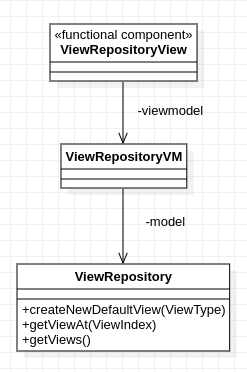
\includegraphics[scale=0.55]{../../assets/classi_uml/viewrepo.png}
  \caption{Implementazione repository}
\end{figure}


% \subsection{Diagrammi dei package}
% \subsection{Diagrammi delle classi}

% \subsubsection{View}

% \begin{figure}[h!]
    % \centering
    % 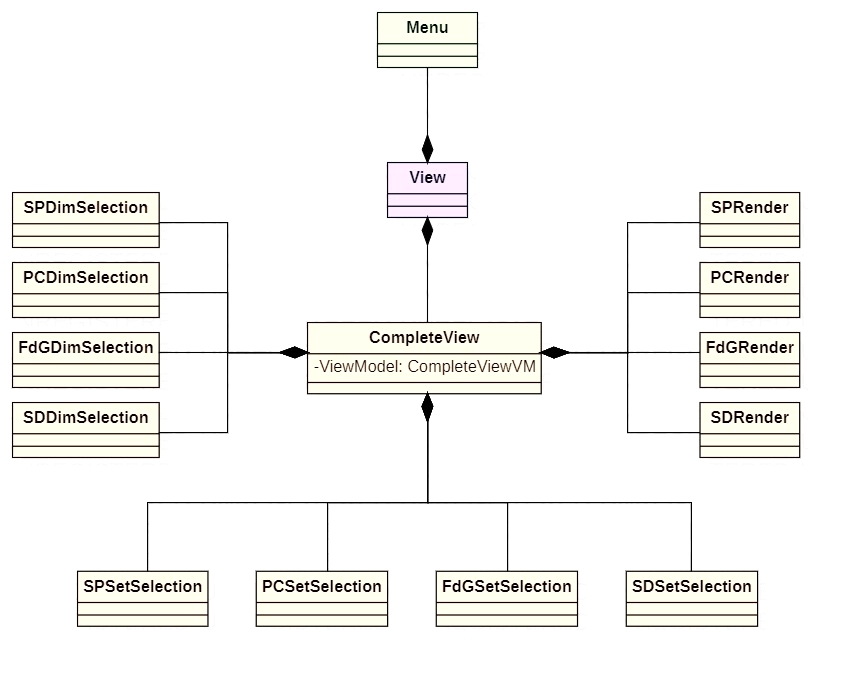
\includegraphics[scale=0.75]{../../assets/classi_uml/View.jpg}
    % \caption{Diagramma delle classi - View}
% \end{figure}
% \newpage
% \subsubsection{Model}

% \begin{figure}[h!]
    % \centering
    % 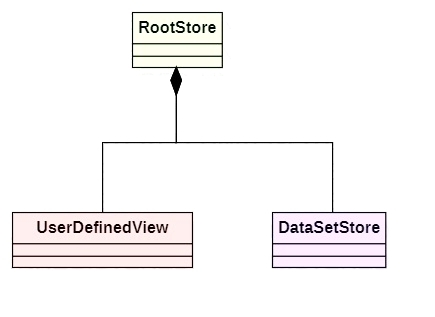
\includegraphics[scale=0.75]{../../assets/classi_uml/Model.jpg}
    % \caption{Diagramma delle classi - Model}
% \end{figure}

% \subsection{Diagrammi di sequenza}
